

\chapter{Pandora's Actor}

\begin{figure}
    \centering
    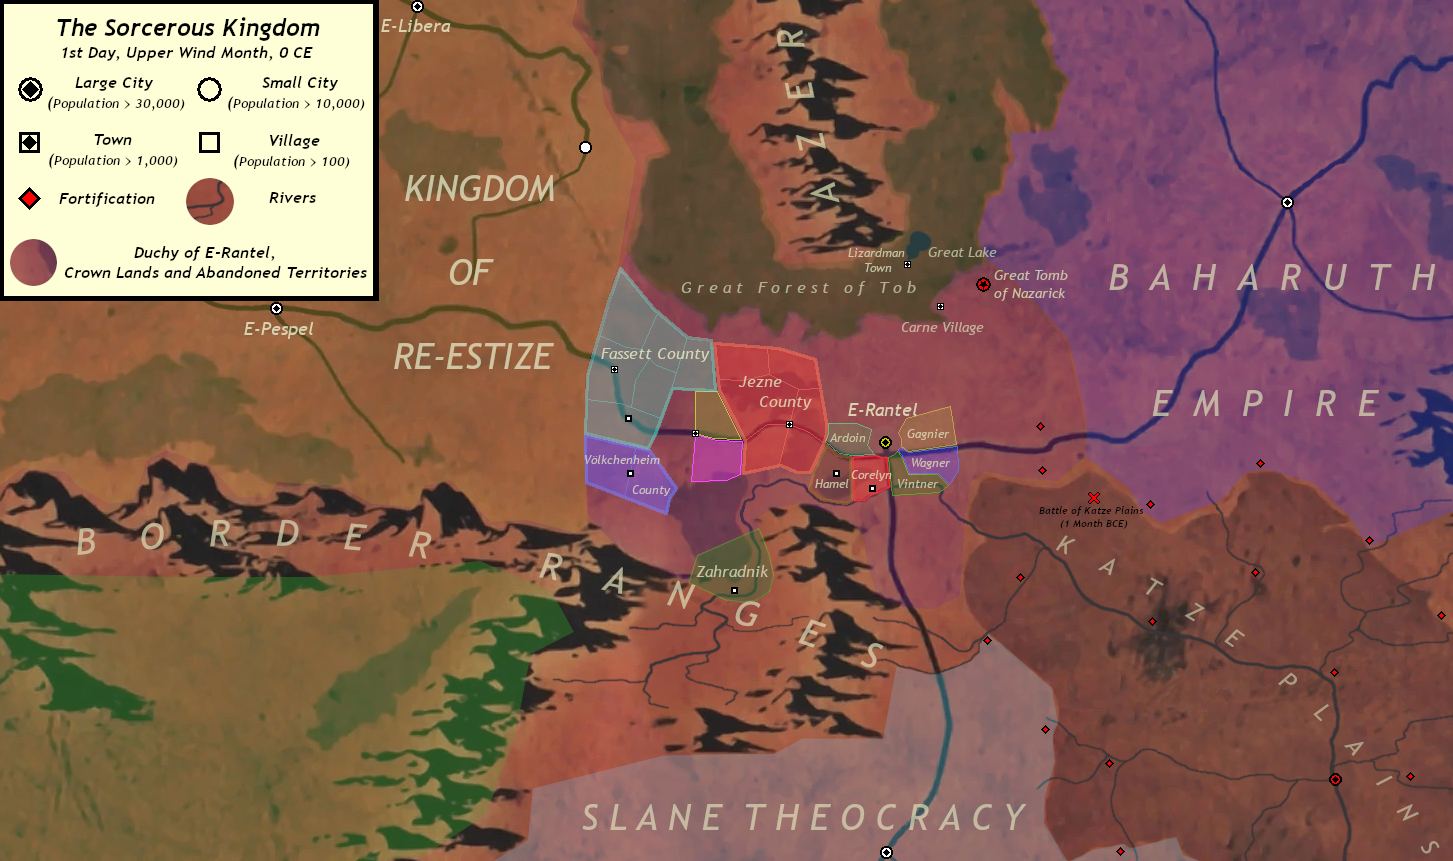
\includegraphics[width=1\linewidth]{images/ViGYZcC.png}
    \caption*{Political Map of the Sorcerer Kingdom}
\end{figure}

"Haaahhh~"


A prodigious sigh arose from behind him. It was a sound filled with equal parts annoyance, frustration and fatigue – as if one’s soul had been stretched thin and would dissipate like their misted breath in the frigid spring air. The drawn-out expression prompted the man to shift his body to look towards his companion: a woman seated astride a handsome mount that trotted after his own.

 

She was dressed plainly, in a clean set of traveller’s garments; wrapped in a brown cloak that tumbled past her horse’s flanks. Silky black hair – which somehow maintained its gleaming lustre despite long days of riding on rough country roads – was tied up in a loose ponytail that lightly streamed back and forth in the morning breeze. In her hands, she grasped an unfurled roll of parchment; her face was painted with an expression of irritation.

 

It gave an edge to her cold beauty, which – much to his own bemusement – had become something of a commodity in itself amongst some of the locals. Had he not known better, he might have assumed that it was the content of the parchment that was the source of her vexation...but he possessed a copy of it as well.

 

It was a map: a rough copy prepared from one that was found filed away in the civil offices of E-Rantel, detailing the southern regions of its duchy.

 

He had seen the original himself – its aged vellum cracked and yellowed despite careful attempts at preservation over the years: a meticulous survey done generations ago when the Kingdom of Re-Estize was near the height of its prosperity.

 

Laid upon it was a burgeoning frontier in the midst of expansion. The primal woodlands of the wilderness had been cleared away to make room for farms and pastures. Aristocratic manors spotted the fiefs on the map, carefully positioned on a network of well-travelled earthen roads. A multitude of hamlets and villages had sprouted up around them, filled with hopeful immigrants from the more populated regions of the Kingdom and beyond – pioneers cultivating the land to build a future of their own.

 

It was a map that spoke of a bright future. It was a time where order ruled and enterprising Adventurers tamed the wild borderlands surrounding the fledgling town that would grow to become E-Rantel, forging the way for settlement and industry. The House of Vaiself put its full support behind the expansion, investing heavily in both manpower and materials. When suitable lands were cleared, new titles were bestowed on those of appropriate merit, and so this cycle continued until the duchy had expanded all the way into the foothills of the border ranges to the south.

 

It was a map made generations ago; yet now, barely a trace of the scenery depicted by its features could be found in their surroundings. But it was not the feeling of betrayed expectations, he knew, that drew the heavy sigh from the woman behind him.

 

If she was aware of his gaze, she did not show any sign of it. She simply continued to scowl at the map as if her glare could ignite the thin piece of paper and scatter its ashes to the wind. Most likely, he mused, she was imagining the inhabitants: Humans, toiling in their simple fields and pastures; milling about in their meagre hamlets and villages. Tens of thousands of Humans squirming across the face of her map like a writhing infestation that threatened to crawl off the parchment, onto her fingers and up her arm.

 

He suppressed a smirk as he turned back around to face forward, though no one could have possibly seen it under the pitch-black metal of his fully-enclosed helm. While he did not exactly empathize with her feelings, as a fellow Doppelganger he understood the root of them.

 

The vast majority of their species nurtured a natural disdain of those not of their own, bordering on a malignant, almost xenophobic hatred. While their place as denizens of Nazarick meant that they got along well enough with fellow servants of the Supreme Beings, it also meant that outsiders earned a double serving of both a Doppelganger's natural ire and the sense that accompanied their existence as wretched, misbegotten creatures: unblessed by the touch of their Creators.

 

Personally, he did not lend himself much to these feelings, but he was still plagued by a mild irritation of a different sort that steadily grew as their journey progressed further.

 

To curb the inevitable wave of citizens fleeing at the news of Re-Estize’s catastrophic defeat on the Katze Plains, they had been immediately dispatched as Momon and Nabe: the Adamantite adventurers of Darkness. Their objective was to calm the rural population with their presence in an effort to stem the tide of refugees from crossing the borders.

 

When they had departed on their mission, gently rolling fields lay fallow through the winter, undisturbed after the autumn harvest. The roads leading west were well worn and everywhere evidence could be seen of rural products having been readied for delivery to the winter markets. Much of it had already disappeared, carried away by the desperate tide.

 

It had seemed like a straightforward task at first; the groundwork for their mission had been laid out by the magnificent foresight of their Master. The fame of Darkness had spread far and wide; their reputation beyond any conceivable reproach. The labourers that still remained around the villages unbent themselves from their labours to cheer and wave as they passed. Wherever they stopped, men and women would gather about them with hope and excitement; whenever they spoke, everyone would give their full attention and support.

 

Many of the wealthiest families in the fiefs that straddled the paved highway leading westward towards the Kingdom seemed to have already gotten wind of recent events and had fled the duchy out of fear, so they spent little time with the accompanying formalities as they visited the towns, villages and hundreds of hamlets spread out over vast stretches of rural land.

 

However, as their journey turned southwards and the days and weeks passed, the farmlands grew more sparse...as did the people supposedly tending to them. Fields and pastures transformed into grassland and meadows dotted with small groves of aspen and other poplars. Eventually, the lands along the roads could no longer be recognized as anything resembling fields and patches of young forest grew more prevalent. The wide, open roads had become little more than shadowed footpaths with sunlight filtering down through gaps in the thick web of branches overhead. At this point in their journey, these roads could just as easily have been mistaken for old animal trails amongst the dense undergrowth but for the fact that they were unnaturally straight.

 

The route that they currently travelled was marked on the map as part of a network of trails wide enough for wagons and carts, crisscrossing the landscape and linking the myriad farming communities leading through to the southern frontier. In reality, however, it had become more and more dilapidated and overgrown the further they travelled.

 

If not for Aura, who had ranged across the area with her own detachment weeks previous and later explained that the map was indeed correct – that the wilderness had simply reclaimed the land over time – he might have written it off as a whimsical fancy concocted by some blustering bureaucrat trapped behind a desk in the city. Even his Creator, who now styled himself Ainz Ooal Gown, marveled at the land's ability to restore itself to its natural state.

 

“Momon-san.”

 

A soft, dispassionate voice from behind roused him from his recollections. He raised his head to scan the surroundings ahead of them. Slightly off the path at the crest of the ridge that they were currently scaling, not ten paces into the forest, a small building stood overgrown and shadowed by creeping vines. It appeared to have sunk into the ground somewhat, or perhaps layers of humus had built up around it over the years.

 

“I see it, Nabe,” he slowed his mount to a stop as his companion followed suit. “What did they find?”

 

As if on cue, a figure materialized out of the dimly-lit undergrowth nearby to Narberal. It was one of the many Hanzos deployed alongside them, combing the terrain ahead as both an escort and a reconnaissance force for their mission. Narberal leaned forward to receive its report with thanks – without their tireless work, covering the entire region would have taken ages.

 

“It’s an old sentry post,” she stated flatly. “Abandoned years ago.”

 

“Umu,” he nodded, urging his mount forward once again.

 

They had come across similar sights all along their journey once they had left the immediate vicinity of E-Rantel. Though some places had been abandoned in fear by their inhabitants and those that ruled over them upon hearing of the Kingdom’s defeat at the hands of the Undead Sorcerer King, most recounted a tale that was decades in the making.

 

The region had seen great growth in the past, but at some point it had begun to stagnate for reasons unknown to the current population. Though she would probably not admit it personally, this concerned the Guardian Overseer and Albedo had gone to great lengths to pore over past tax and census records in an effort to discover the cause. She could only infer that when the region had grown to a certain size, the resources and manpower used to expand the Kingdom’s territory had to be diverted towards policing and maintaining the land and its influx of immigrants.

 

Over a stack of old archival tomes, she explained how after the first generation of settlers passed their lands on to their descendants, their burdens began to pile up at an ever accelerating rate. Expenditures for security against monsters, Demihumans and bandits grew until they could no longer be maintained by taxation. The militia could only man the largest of population centres and adventurers could only be afforded as a stopgap measure against the most apparent and dire of threats. Roads became wrought with hazards and commerce slowed to a crawl as the dangers increased. With the land no longer safe and prosperous, immigration had ground to a halt. Over the years, outlying settlements were abandoned in turn until only nature was left to reclaim what had been taken from it.

 

“Those inferior lifeforms should have never crawled out of their holes,” Albedo’s words dripped with equal parts venom and disdain. “No matter what they may aspire to, worms will always be worms: destined to squirm beneath the ground.”

 

This slow and steady decay continued until the present day, where they bore witness to the dismal end of the tale. As both the Guardian and curator of Nazarick’s treasury, it both shocked and appalled him that the Kingdom could let its territory and possessions reach such a decrepit state. What had initially been irritation slowly rose to anger within him at the sight of every abandoned farm and village; every rusted plough and collapsed cottage. He continued to fume as he looked upon the painstakingly laid out network of run-down roads choked by vegetation with their aged sentry towers fallen into disrepair and ruin.

 

At one point he had imagined the Great Tomb of Nazarick in such a state and it filled him with such fury that even Narberal, who was often teased for being oblivious by her sisters, could feel the rage emanating from him and surreptitiously scurried further down the trail – though she never knew exactly why.

 

Shortly thereafter, he reined in his feelings on the matter so Narberal would stop shying away from him, though they still simmered beneath the surface somewhere. He consoled himself with the fact that this land was now under the dominion of Ainz Ooal Gown, and under his Master’s guidance and protection it would soon be vaulted beyond its former glory and fashioned into something suitable enough to be called a possession of the Supreme Beings.

 

“Furthermore,” Narberal continued, “the settlement at the end of the trail still seems to be intact and occupied.”

 

Pandora’s Actor, who had fallen to brooding at the first piece of news, looked once again to the crest of the ridge with interest.

 

“Hoh…” this was unexpected, indeed. “So at the end of all these ruined farmsteads and forgotten paths, something still stands? Let us see what manner of people can endure where all others have failed.”

 

Articles both valuable and remarkable were of keen interest to Pandora’s Actor. Like his creator, he was a collector; the idea that something unprecedented lay just beyond the next hill was a tantalizing thought with the otherwise unremarkable journey that they had made. Though nothing in this world that he had witnessed so far could hope to compare to what lay within the vaults of Nazarick, to discover articles both exotic and rare – to catalogue and ascertain their value – was a pleasure in and of itself.